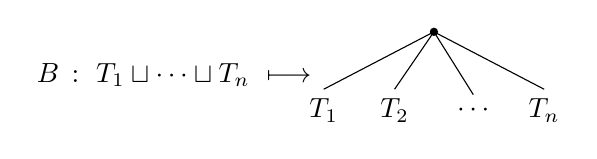
\begin{tikzpicture}
\node at (-1.9,-0.45) {$\mathfrak{B}\,:\ T_1\sqcup\cdots\sqcup T_n\ \longmapsto$};
\coordinate (r) at (1.4,0.1);
\node (t1) at (0,-0.9) {$T_1$};
\node (t2) at (0.9,-0.9) {$T_2$};
\node (td) at (1.9,-0.9) {$\cdots$};
\node (tn) at (2.8,-0.9) {$T_n$};
\draw (r) -- (t1.north); \draw (r) -- (t2.north); \draw (r) -- (td.north); \draw (r) -- (tn.north);
\fill (r) circle (1.5pt);
\end{tikzpicture}
